\subsection{Subsystem $<$Util$>$}

\subsubsection{Detailed Design Diagram}
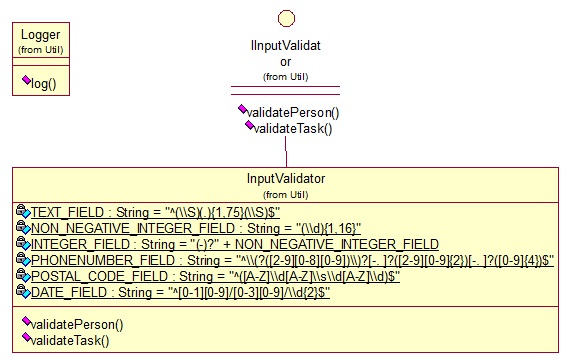
\includegraphics{subsystems/diagrams/utils_class_diagram}

This package stores all the utility classes needed in the application. Utility classes are classes that are required in multiple components of the application. It contains the Logger, IInputValidator and InputValidator classes.

\subsubsection{Units Description}

\emph{Logger}\\
Functions:\\
\begin{tabular}{| l | l | l | l |}
\hline
Name & Parameters & Pre-conditions & Post-conditions\\
\hline
\multirow{2}{*}{log} & String className, String log & Requires Nothing & Logs \emph{className} and \emph{log} parameters to console
\\&  & & and passed to the main view
\\
\hline
\end{tabular}
\\

Attributes: \emph{none}
\\

Purpose: Its purpose is to log to console the message provided to it. The advantage of a Logger versus directly outputting to console via \emph{System.out.println()} is that it can easily be extended to log to a file without having to made code chage to anywhere else in the application.
\\
\\
\emph{IInputValidator}\\
Functions:\\
\begin{tabular}{| l | l | l | l |}
\hline
Name & Parameters & Pre-conditions & Post-conditions\\
\hline
\multirow{2}{*}{view} & JXPathContext personNode       & Requires the JXPathContext	&  Validates the tasks and\\							
			 & JXPathContext taskNode           & pointer to a valid location.        & people from the xml file
\\
\hline
\end{tabular}
\\

Purpose: Describe the interface for validating the xml input.
\\
\\
\emph{InputValidator}\\
Functions:\\
\begin{tabular}{| l | l | l | l |}
\hline
Name & Parameters & Pre-conditions & Post-conditions\\
\hline
\multirow{2}{*}{view} & JXPathContext personNode       & Requires the JXPathContext	&  Validates the tasks and\\							
			 & JXPathContext taskNode           & pointer to a valid location.        & people from the xml file
\\
\hline
\end{tabular}
\\

Attributes:\\
\begin{tabular}{| l | l |}
\hline
 Name                                                        & Description\\
\hline
String NON\_NEGATIVE\_INTEGER\_FIELD  & REGEX match for non-negatif integers to validate IDs\\
\hline
String INTEGER\_FIELD                               & REGEX match for integers to validate IDs\\
\hline
String PHONENUMBER\_FIELD                    & REGEX match to validate phone numbers\\
\hline
String POSTAL\_CODE\_FIELD                    &  REGEX match to validate postal codes\\
\hline
String DATE\_FIELD                                    &  REGEX match to validate dates\\
\hline
\end{tabular}\\
\\

Purpose: Its purpose is to validate XML inputs before loading the data into objects to ensure the stability of the application.
\\
\\